\documentclass{article}

\usepackage[a4paper,margin=3cm,headsep=1cm]{geometry}
\usepackage[utf8]{inputenc}
\usepackage{%
    booktabs,
    fancyhdr,
    pgfgantt,
    titlesec,
    clrscode3e,
    exercise,
    tikz,
    subcaption
}
\usetikzlibrary{trees}

\pagestyle{fancy}

\rhead{Algorithms and Data Structures, S25}
\lhead{Exercises part 1, Lecture 04}
\rfoot{Aalborg University, Copenhagen}
\lfoot{Andreas Holck Høeg-Petersen}

\begin{document}
\thispagestyle{fancy}

\begin{Exercise}[title={Stacks and queues}]

    \Question
    Using Figure 10.2 as a model, illustrate the result of each operation in the
    sequence $\proc{Push}(S,4)$, $\proc{Push}(S,1)$, $\proc{Push}(S,3)$,
    $\proc{Pop}(S)$, $\proc{Push}(S,8)$ and $\proc{Pop}(S)$ on an initially
    empty stack $S$ stored in array $S[1:6]$ (CLRS 10.1-2)

    \Question
    Using Figure 10.3 as a model, illustrate the result of each operation in the
    sequence $\proc{Enqueue}(Q,4)$, $\proc{Enqueue}(Q,1)$,
    $\proc{Enqueue}(Q,3)$, $\proc{Dequeue}(Q)$, $\proc{Enqueue}(Q,8)$ and
    $\proc{Dequeue}(Q)$ on an initially empty queue $Q$ stored in array $Q[1:6]$
    (CLRS 10.1-4)

    \Question
    Show how to implement a queue using two stacks. Analyze the running time of
    the queue operations. (CLRS 10.1-7)

\end{Exercise}

\begin{Exercise}[title={Linked lists}]
    \Question
    Explain why the dynamic-set operation $\proc{Insert}$ on a \textit{singly}
    linked list can be implemented in $O(1)$ time, but the worst-case time for
    $\proc{Delete}$ is $\Theta(n)$. (CLRS 10.2-1)

    \Question
    Implement a stack using a \textit{singly} linked list. The operations
    $\proc{Push}$ $\proc{Pop}$ should still take $O(1)$ time. Do you need to add
    any attributes to the list? (CLRS 10.2-2)

    \Question
    Give a $\Theta(n)$-time nonrecursive procedure that reverses a singly linked
    list of $n$ elements. The procedure should use no more than constant storage
    beyond that needed for the list itself. (CLRS 10.2-5)
\end{Exercise}

\begin{Exercise}[title={Heaps}]

    \Question
    What are the minimum and maximum numbers of elements in a heap of heigh $h$?
    (CLRS 6.1-1)
    
    \Question
    Is an array that is in sorted order a min-heap? (CLRS 6.1-5)

    \Question
    Are the trees below valid max-heaps? Why / why not?

    \Question
    Is the array with values $\langle 33, 19, 20, 15, 13, 10, 2, 13, 16, 12
    \rangle$ a max-heap? (CLRS 6.1-7)

    \Question
    Show that, with the array representation for storing an $n$-element heap,
    the leaves are the nodes indexed by $\lfloor n/2 \rfloor + 1$, $\lfloor n/2
    \rfloor + 2$, \ldots, $n$. (CLRS 6.1-8)

\end{Exercise}

\begin{figure}[h]
    \begin{subfigure}{.45\textwidth}
        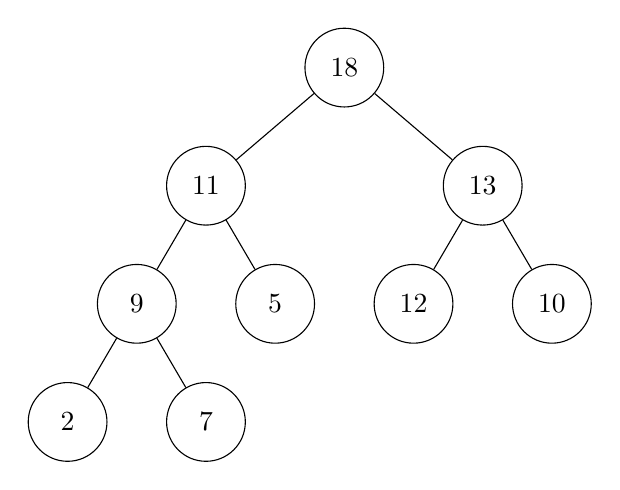
\begin{tikzpicture}[
            level distance=1.5cm,
            level 1/.style={sibling distance=10em},
            level 2/.style={sibling distance=5em},
            every node/.style={draw, circle, minimum size=1cm}]
            \node {18}
                child {node {11}
                    child {node {9} 
                        child {node {2} }
                        child {node {7} }
                    }
                    child {node {5} }
                }
                child {node {13}
                    child {node {12} }
                    child {node {10} }
                };
        \end{tikzpicture}
        \caption{}
    \end{subfigure}
    \hfill
    \begin{subfigure}{.45\textwidth}
        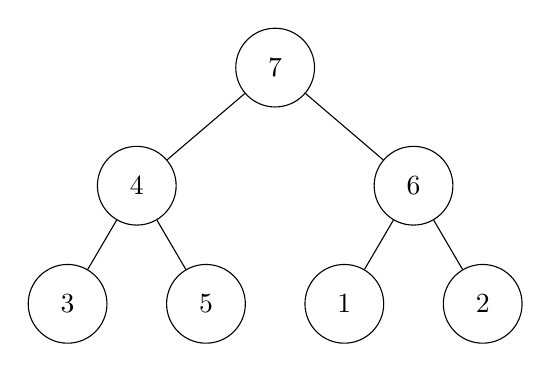
\begin{tikzpicture}[
            level distance=1.5cm,
            level 1/.style={sibling distance=10em},
            level 2/.style={sibling distance=5em},
            every node/.style={draw, circle, minimum size=1cm}]
            \node {7}
                child {node {4}
                    child {node {3} }
                    child {node {5} }
                }
                child {node {6}
                    child {node {1} }
                    child {node {2} }
                };
        \end{tikzpicture}
        \caption{}
    \end{subfigure}
\end{figure}

\end{document}

